\documentclass[11pt,a4paper]{article}

\setcounter{secnumdepth}{6}

\usepackage{standalone}

\usepackage{geometry} % Used to adjust the document margins
%~ \geometry{bindingoffset=1cm}
\usepackage{fullpage}
\usepackage{multirow}
%~ \usepackage{wasysym}
\usepackage{setspace}
\doublespacing

\usepackage{graphicx}
\usepackage[font=footnotesize]{caption}
\usepackage[noadjust]{cite}
\usepackage[toc,page]{appendix}
\usepackage{hyperref}


\usepackage{amsmath}
\usepackage{amsfonts}

%~ \usepackage{sidecap}
\usepackage{caption}
\usepackage{subcaption}


\usepackage[colorinlistoftodos,disable]{todonotes}
%~ \usepackage[colorinlistoftodos]{todonotes}
\usepackage{csquotes}
\usepackage{parskip} % Spaces between paragraphs


\usepackage[acronym]{glossaries}
% add binding margins


\makeglossaries

%~ \renewcommand*\abstractname{Summary}

% http://www.tex.ac.uk/cgi-bin/texfaq2html?label=altabcr
\setcounter{MaxMatrixCols}{50}

% package name:
\newcommand{\py}{\texttt{python}}
\newcommand{\pr}{\texttt{pyrem}}
\newcommand{\pyeeg}{\texttt{PyEEG}}
\newcommand{\ctit}{\emph}
\newcommand{\ptit}{\emph}

\newcommand{\eg}{\emph{e.g.}}
\newcommand{\ie}{\emph{i.e.}}

\newcommand{\specialcell}[2][c]{\begin{tabular}[#1]{@{}c@{}}#2\end{tabular}}


\newcommand{\FIXME}[2][]{\todo[color=cyan, #1]{\textbf{QG:} #2}}
\newcommand{\TODO}[2][]{\todo[color=red, #1]{\textbf{QG:} #2}}

\newcommand{\citationneeded}[2][]{\todo[color=brown, fancyline, #1]{\textbf{Citation Needed:} #2}}
\newcommand{\contrib}{\emph}
\begin{document}

\pagenumbering{roman}

\title{abcd}
\author{Quentin Geissmann\\
\\	
\\
\\
\\
Supervised by Giorgio Gilestro\\
\\
\\
Imperial College London
}
\date{\today}

\clearpage\maketitle
\thispagestyle{empty}
\newpage{}

\listoftodos
\newpage



% our acronyms
\newacronym{rem}{REM}{Rapid Eye Movement}
\newacronym{nrem}{NREM}{Non-Rapid Eye Movement}
\newacronym{eeg}{EEG}{Electroencephalogram}
\newacronym{emg}{EMG}{Electromyogram}
%~ \newacronym{eog}{EOG}{ElectroOculoGram}
\newacronym{svm}{SVM}{Support Vector Machine}
\newacronym{ann}{ANN}{Artificial Neural Network}
\newacronym{hmm}{HMM}{Hidden Markov Model}

%~ 
%~ \newglossaryentry{epoch}
%~ {
  %~ name=epoch,
  %~ description={todo
   %~ },
  %~ sort = epoch
%~ }
%~ 
%~ \newglossaryentry{$fs$}
%~ {
  %~ name=fs,
  %~ description={Samplig frequency
   %~ },
  %~ sort = fs
%~ }



\begin{abstract}

Electroencephalography (EEG) is a very widespread technique which is routinely used
as a diagnostic tool for brain dysfunctions and to investigate neurological
phenomenons.
Because of its relatively non-invasive nature,
it is widely used to determine and quantify sleep stages in humans and model
mammals such as rodents.
Historically, labelling of EEG recordings has been performed visually by trained
human experts. This task is extremely tedious and quite subjective.   
Despite recent efforts to develop an automatic classifier of sleep stages,
little adoption has occurred, and manual scoring is still the standard.

This study presents a high accuracy classifier of sleep stages that
could lead to an efficient software tool for biologists.
Exhaustive feature extraction based on discrete wavelet decomposition was used
in combination with a random forest classifier and was demonstrated to achieve
an overall accuracy of as high as 92\%.
In order to optimise feature extraction and pave the way for a future software
implementation, \pr{}, a \py{} package was also developed. \pr{} is here shown
to outperform an alternative runtime implementation by several orders of magnitude.
	\\
	\\
\begin{itemize}
\item Words in main text: 4996
\item Words in headers: 84
\item Words outside text (captions, etc.): 943
\end{itemize}
%~ 
\end{abstract}

\newpage

\tableofcontents
\newpage
\printglossaries

\newpage
\pagenumbering{arabic}

\section{Introduction} \label{intro}
\TODO{fig 2: rasterize}
\TODO{fig 2: smaler coeff text}
\TODO{remover a lot from mat and met}
\TODO{fix he large number of subsecions}
\TODO{fix benchmark table reorder}
\TODO{wake vs awake}
\TODO{conclusion should do more  justice}

Sleep is considered to be a ubiquitous and necessary behaviour amongst
animals\cite{siegel_all_2008,cirelli_is_2008}.
However, its real physiological functions remain debated.
In vertebrate, electrophysiological recordings, in particular, \gls{eeg};
the recording of the global electrical activity in the brain,
but also \gls{emg}, which records muscular activity,
have extensively used to study the structure of sleep during the last
century\cite{loomis_distribution_1938,aserinsky_regularly_1953}.
They have the advantage of being non-invasive an relatively high throughput.
Today, \gls{eeg} remains one of the main asset in the study sleep physiology.

Rodents, in particular mice and rats, have proved very successful model for
understanding of the mechanisms of sleep in mammals\cite{toth_animal_2013}.
Classically, three main distinct types of sleep related behaviours: wakefulness, \gls{nrem} sleep and \gls{rem} 
sleep are referred as \emph{vigilance states}.
Vigilance states are usually defined on the basis of \gls{eeg} and \gls{emg} (fig.~\ref{fig:sleep_description}).
When awake (WAKE), animals tend to have a high muscular activity which translates as a high amplitude voltage changes in the \gls{emg}.
During wakefulness, \gls{eeg} is dominated by a relatively low amplitude oscillations of frequency
between six and ten hertz often referred as theta waves.
In contrast, \gls{nrem} sleep, also called slow wave sleep, is a period of muscular inactivity (low \gls{emg})
dominated by slow oscillations (below 4Hz) of high amplitude named delta waves.
The third state, \gls{rem} sleep, is characterised by a complete lack of muscular activity (atony) and an \gls{eeg} activity very similar to the awake state.
\gls{rem} sleep is the least prevalent of all three stages, and represents generally  20\% of all sleeping time.
The prevalence of these three states as well as their temporal organisation are extremely important observations in sleep research


\begin{figure}[h!]

  \centering    
    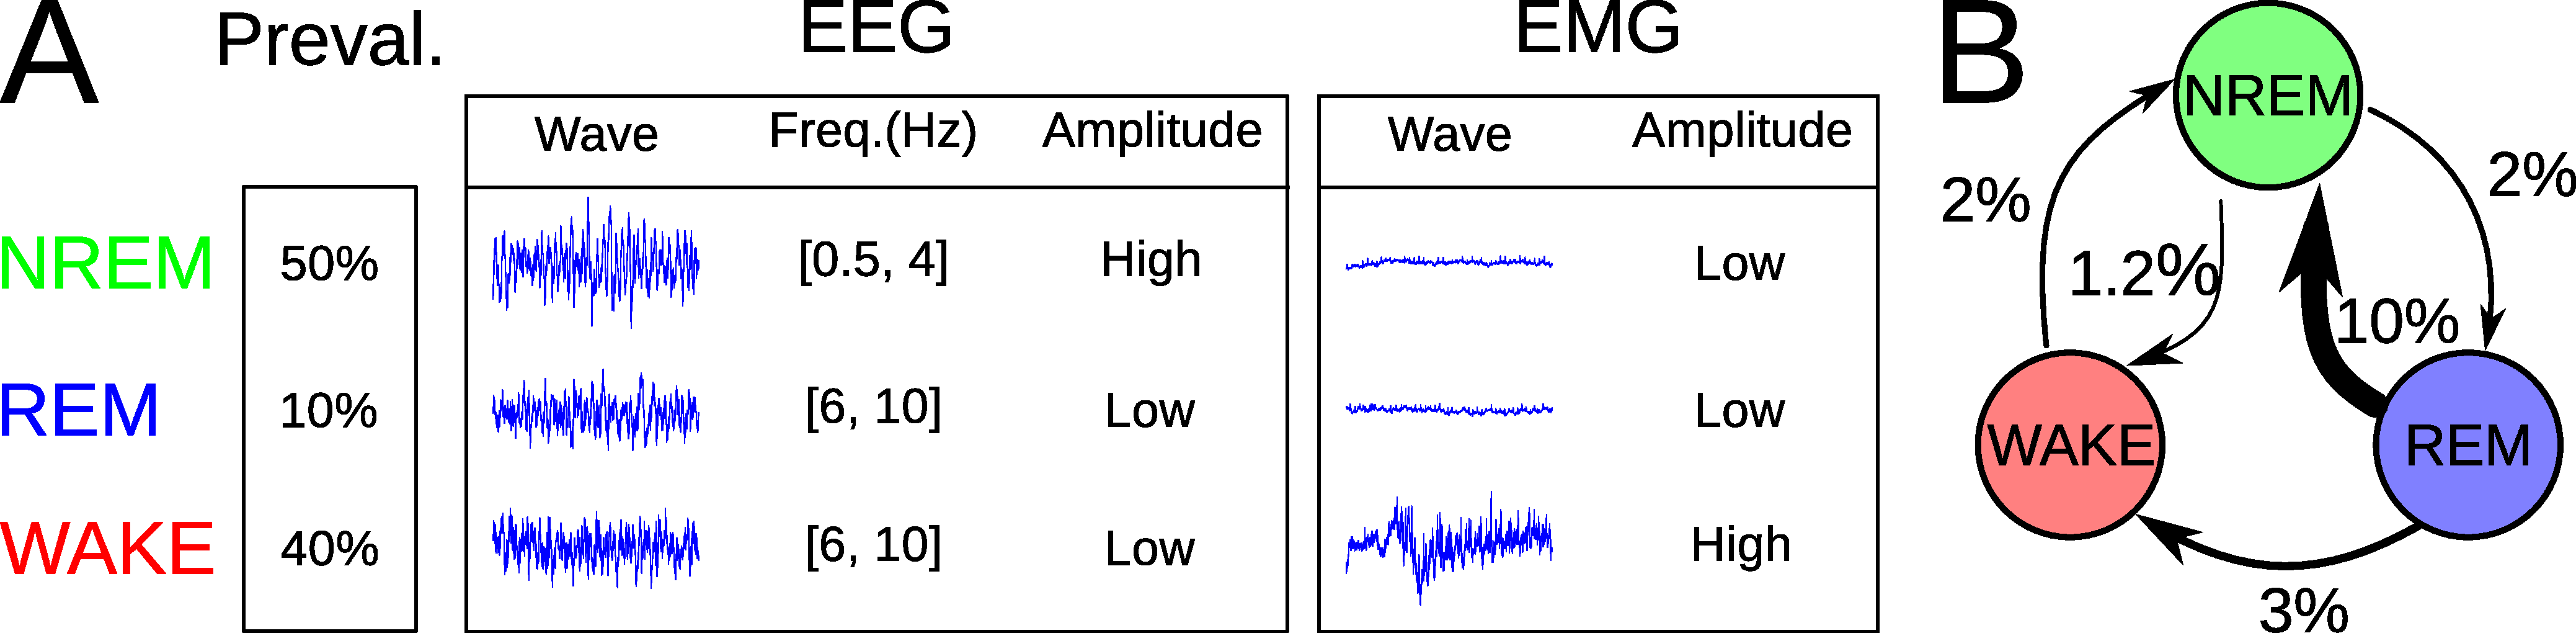
\includegraphics[width=0.95\textwidth]{figures/sleep_description.pdf}
  \caption{\ctit{Structural description of sleep stages.}
  \textbf{A}: Characteristics of the three sleep stages.
  Typically, frequency and amplitude of the \acrfull{eeg}, and amplitude of the \acrfull{emg} are used by experts to infer sleep stage.
  The presented frequency ranges and and pevalences are approximate values for healthy adult animals in normal conditions.
  Each wave shows a representative five second epoch with high signal to noise ratio.
  \textbf{B}: Empirical transition probabilities between consecutive five second epochs. The width of the arrow is proportionnal to the probability of transition.
  Probabilities of remaining in the three state are implied.
  \label{fig:sleep_description}
  }
           
\end{figure}



Although definitions of sleep stages appear straightforward, in practice, many cases are ambiguous.
For instance, it is difficult to characterise transitions between two states.
In addition, there are many sources of variability including how surgery was performed, the type of instrument used and inter-animal variability.
The quality of the acquisition can also be made considerably worst by noisy signals or by the presence of artefacts.
For these reasons, sleep scoring, \ie{} the attribution of discrete vigilance states to electrophysiological time series,
is traditionally performed by trained human experts.
Such manual annotation is very time consuming; several hours of work have been reported in order to score 24h of recording.
This severely limits data throughput, and human subjectivity is likely to introduce systematic bias.
Indeed, it is expected that scoring will be performed differently by each expert, making result difficult to reproduce independently.
Often, two experts score the same data, in order to ensure satisfying agreement.
Although, manual scorers are generally reported as being very consensual with
each other\cite{costa-miserachs_automated_2003,sen_comparative_2014}, it can be
argued that experts most likely work in the same laboratory and trained one another, or were trained by the same third person.
In this context, agreement between experts does not account for the variability between communities of researchers, and cannot be used to assess reproducibility.

In order to overcome both speed and subjectivity limitations, efforts have long
been directed towards automation of sleep
scoring\cite{chouvet_automatic_1980, haustein_automatic_1986}.
However, little adoption has occurred and very few available implementations, in the form of software that biologists could use, have been developed.
Typically, two different approaches to classification have been followed: unsupervised or supervised learning.

Unsupervised learning \cite{langkvist_sleep_2012,sunagawa_faster:_2013} has the
advantage of making no assumption about the nature of the different vigilance states, and how they should be defined.
Therefore, this approach can lead to the discovery of truly new states.
One issue is that the choice of the variables used for clustering is very
critical.
Often, variables such as frequency domain variables are in fact chosen in order
to generate clusters that will match human defined clusters.
In addition, unsupervised methods may lack robustness\cite{sunagawa_faster:_2013} in so far as the
cannot easily include covariates explaining, for instance, variability between recording equipments.

Another approach is to assume human annotations are, although imperfect, biologically relevant and generally consistent,
 and therefore to use supervised learning
 techniques\cite{crisler_sleep-stage_2008,ventouras_performance_2012,doroshenkov_classification_2007,pan_transition-constrained_2012,sen_comparative_2014}.
  Of course, if human decisions were biased, such a method may suffer from the same bias.
However, a vast corpus of experimental work has provided hypothesis about function of these states which tends to validate the actual `existence' of these discrete vigilance states.
Building a classifier that would produce a consensual prediction of vigilance states could be seen as an attempt to formalised and rationalise the definition of such states.
This would improve future research without denying decades of sleep neurobiology.

Many supervised learning techniques such as from
\glspl{svm}\cite{crisler_sleep-stage_2008},
\glspl{ann}\cite{ventouras_performance_2012},
to
\glspl{hmm}\cite{doroshenkov_classification_2007,pan_transition-constrained_2012} have been investigated.
In general, the first step is to compute features on consecutive segments of annotated electrophysiological signals know as epochs.
Then, the relation between the response variable(annotation) and the independent variables (features) can be modelled.
Either epochs are considered to be independent from one another or time-dependent structures are explicitly modelled (\eg{} using \glspl{hmm}).
Time aware modelling has the advantage of accounting for the interdependence of consecutive epochs (see fig.~\ref{fig:sleep_description}B).
However, it generally does not model non-linear relationships between large numbers of predictors as well as classical classifiers.

Recently, promising results were obtained for automatic scoring of human sleep stages by performing an exhaustive
feature extraction, including variables resulting from discrete wavelet
decomposition\cite{sen_comparative_2014}.
Then, the authors compared several classifiers and found that random
forest\cite{breiman_random_2001} were, overall, the most accurate predictors.

The study herein bases itself on these promising results by computing an even larger number of features.
An important addition was the computation of time-aware
features\cite{dietterich_machine_2002,deng_time_2013} which significantly improved
accuracy.
Furthermore, rigorous stratified cross-validation\cite{ding_querying_2008} procedure and
comparisons of sleep structure were performed.
These improvement altogether contributed to achieve a very satisfying overall accuracy of 92\%.
In order to pave the way to an implementation of an ubiquitous sleep scoring software.
\pr, a new \py{} package was also build to facilitate efficient feature extraction.
This new package is here demonstrated to be significantly more performance than alternative implementation.


\newpage{}
\section{Material and Methods} \label{matmet}

\subsection{Data}

\subsection{Preprocessing}

\gls{eeg} and \gls{emg} signals were resampled from approximately 200.0Hz to 256.0Hz using
conservative sinc interpolation\citationneeded{Putman}.
A sampling frequency of $f_s  = 256.0Hz$ is convenient since is implies that discrete wavelet decomposition (see subsection~\ref{sub:features} and fig.~\ref{fig:dwd}) will separate
frequencies above 4.0Hz from those below 4.0Hz (since $4 = 256.0/{2^6} $).
This frequency is typically uses as a cut-off value between theta and delta waves \citationneeded{}.
In addition, \gls{eeg} and \gls{emg} signals were standardised ($E[x] = 0, Var[x] = 1$) to account for the variability in baseline amplitude due to acquisition.
Vigilance state anotations were resampled at exactly 0.20Hz using nearest neighbour interpolation.

\subsection{Feature extraction}
\label{sub:features}

A wavelet transform based feature extraction strategy was adopted.
In summary, discrete wavelet decomposition was used on both \gls{eeg} and \gls{emg}
in order to separate frequency bands (fig.~\ref{fig:dwd}).
Then all features were computed on five second epochs for all wavelet coefficients as well as raw signals.

\begin{figure}[h!]
  \centering   
    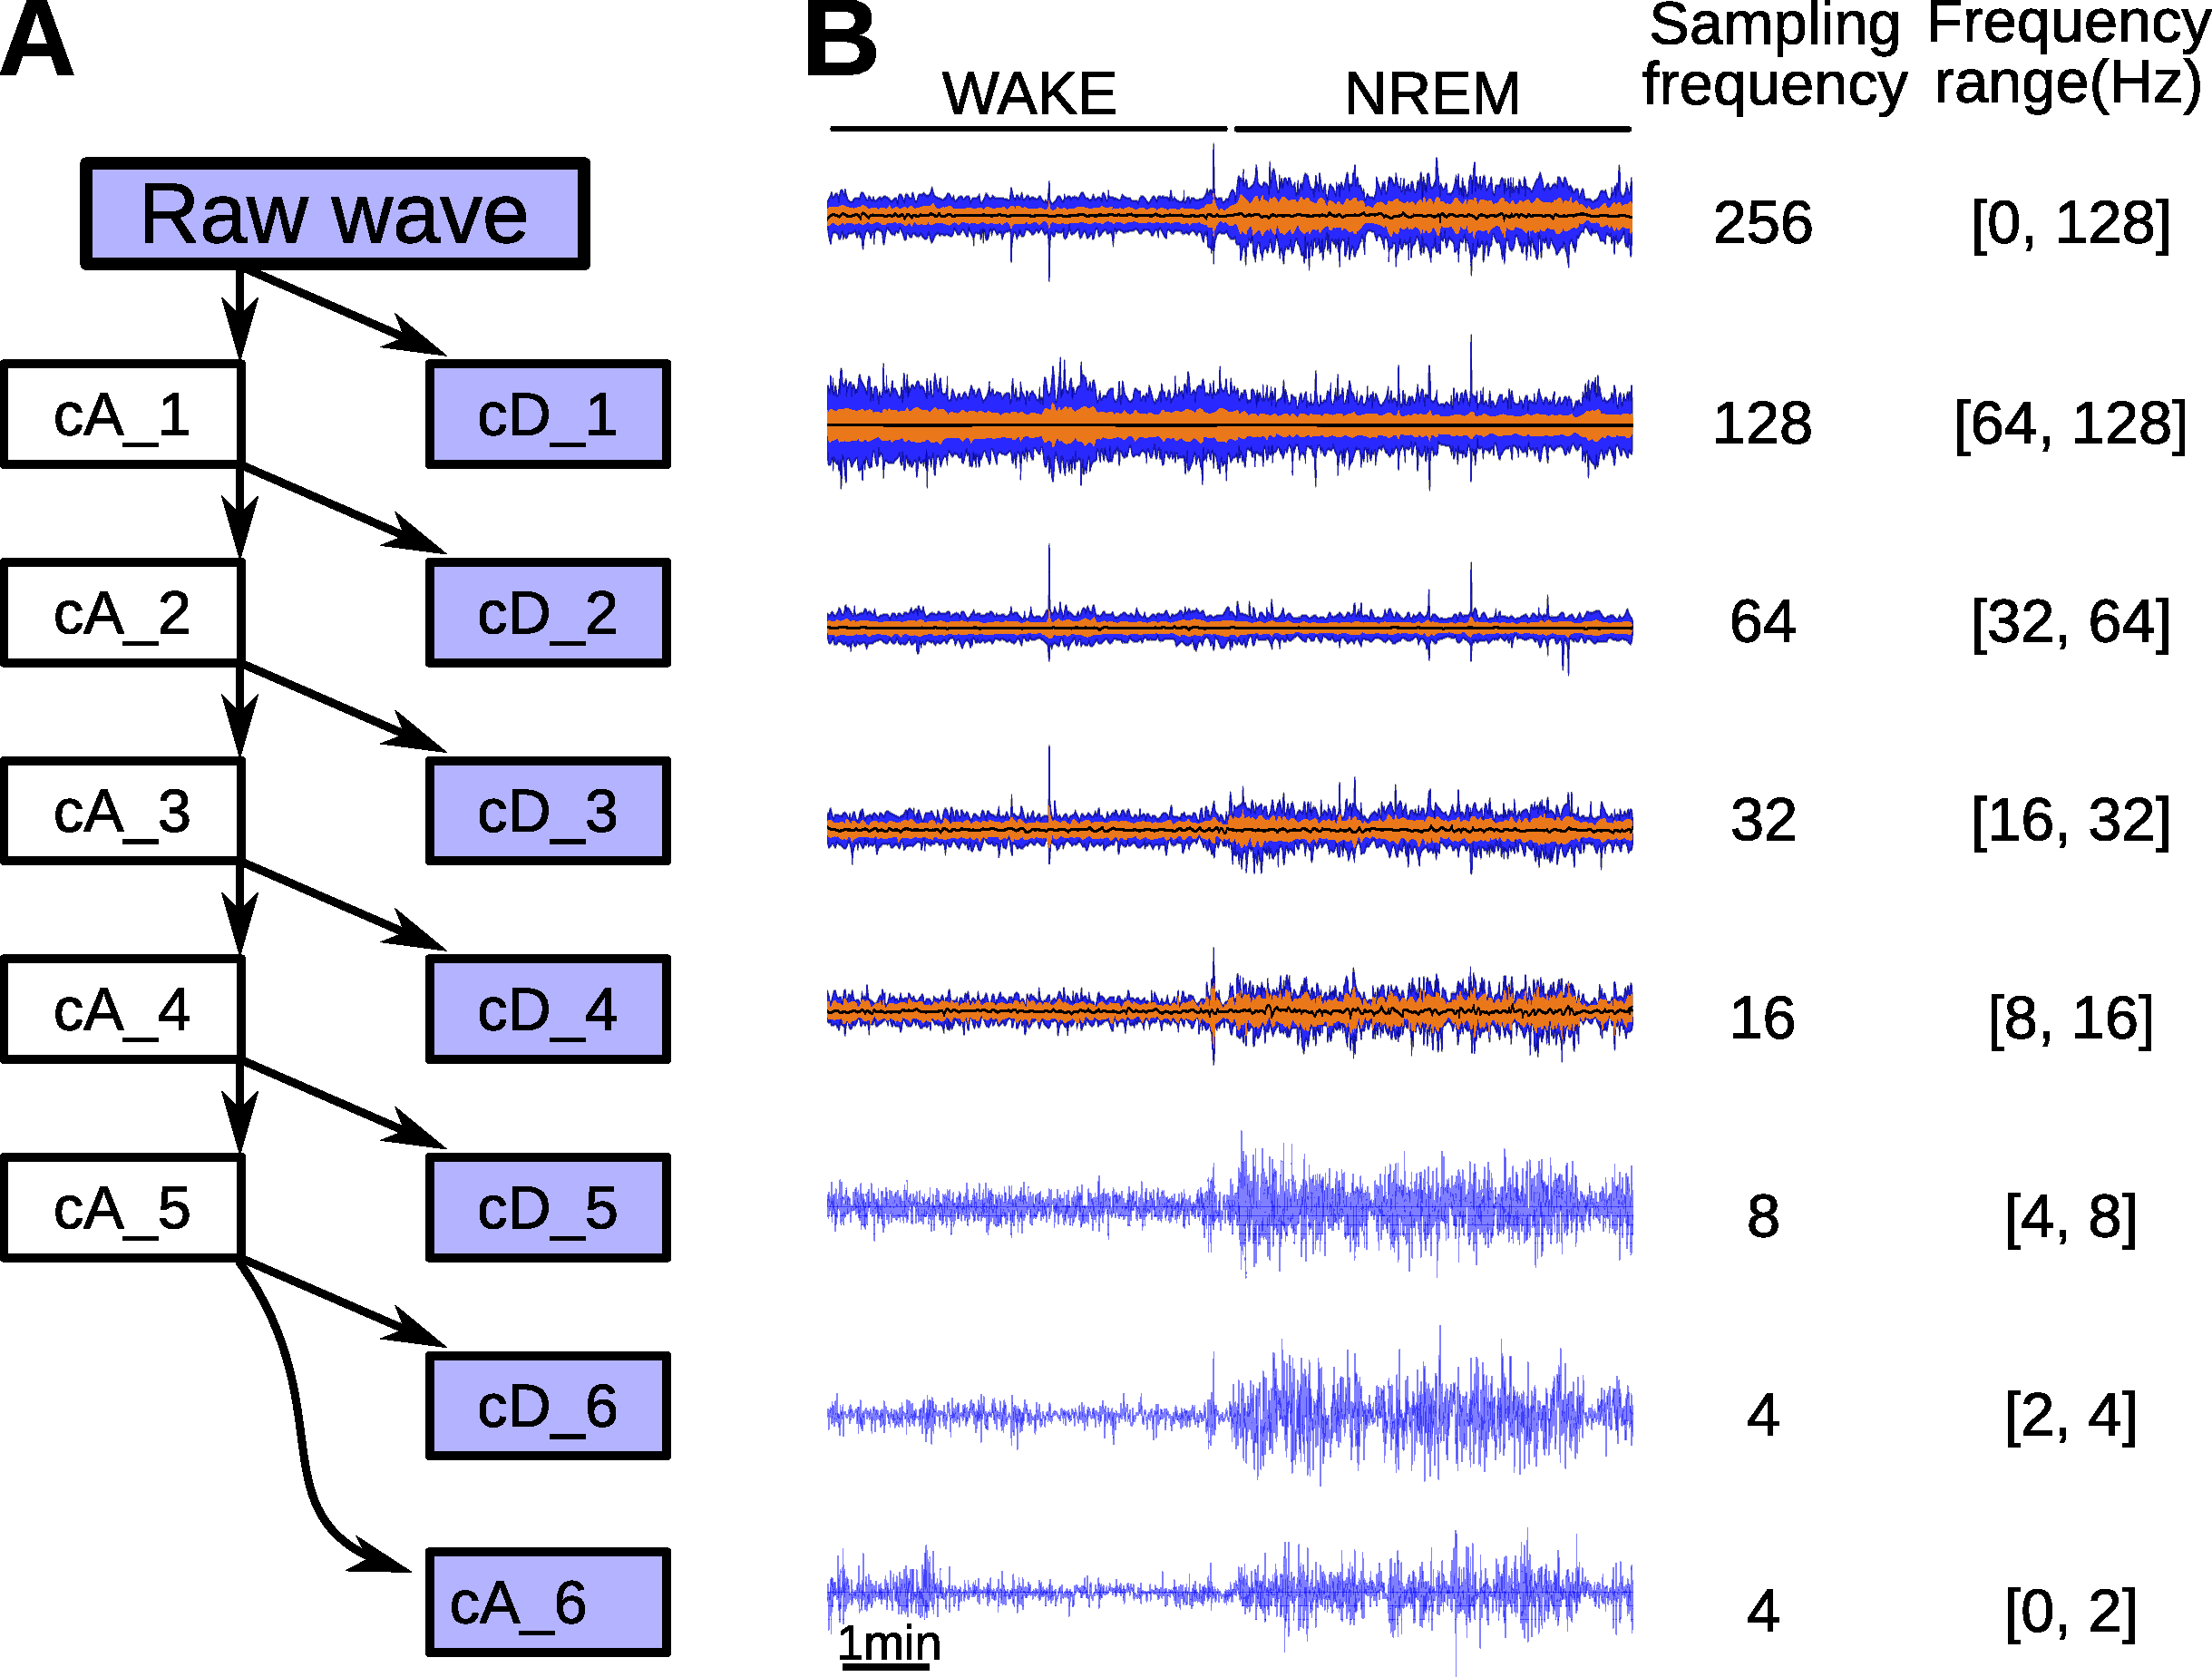
\includegraphics[width=0.95\textwidth]{figures/dwd.pdf}
  \caption{\ctit{Discrete wavelet decomposition.}
	\textbf{A}, Through discrete wavelet transform the initial signal is split into a pair of coefficients: $cA$ and $cD$, which capture the low ($[0, f_s/2]$), and high $[f_s/2, f_s]$ frequency information, respectively.
	Then, discrete wavelet transform is applied iteratively on subsequent $cA$ coefficients ($cA\_1, ..., cA\_n$), thus generating ($cD\_1, ..., cD\_n$).
	In this example, decomposition is performed up to the sixth level ($n=6$).
	\textbf{B}, 
	Ten minutes representing the \gls{eeg} of a transition between a wake and a slow wave sleep(NREM) are shown for the raw
	 wave and for each of the coefficients that are kept for feature extraction (blue rectangles in A).
	 The variation of amplitude in each coefficient corresponds to a concomitant variation of amplitude in the frequency range of this coefficient.
	 In this example, the general increase in power in the raw wave corresponds to an increase of power in the frequency bands below 32Hz, but with a decrease in power above 64Hz.
	%~ Later, each of the eight time series will be segmented into five second epochs, and features are computed for all epochs in the wavelet coefficients and the  raw signal.
	In this figure, the five first signals are too dense to be rendered in a usual fashion. Instead, only local range(blue), inter-quantile range (orange) and median (black line) are represented.
  \label{fig:dwd}
  }
\end{figure}







Importantly, discrete wavelet decomposition was applied \emph{a priory} to the whole signals.
This contrasts with applying decomposition to each epoch \citationneeded{}.
The latter method results in edge effects which would typically need to be attenuated by convolving every epoch with a window function (\eg{} Hamming window).
The maximum decomposition levels for the \gls{eeg} and \gls{emg} signals were six and four, respectively.
Daubechies wavelet, with four vanishing moments (``db4'') was used.

Discrete wavelet decomposition generated seven and five additional time series for \gls{eeg} and \gls{emg}, respectively.
Time series generated from wavelet decomposition (\ie{} coefficients) contain information relative to exclusive frequency sub-bands.
For all 14 time series, a list of 16 features (see table~\ref{tab:features}) was computed in each subsequent non-overlapping five seconds epochs.
Thus, resulting in a total of $p=192$ variables. For each recording ($\simeq 24h$) there were approximately $17000$ epochs.
Some combinations of variables and signals were however incalculable.
These were therefore removed; resulting in an actual number of variables $p=164$.



\begin {table}[!h]
\begin{center}
\caption{\ctit{List of features.}
For clarity, features were classified in four functionnal families.
16 scalar features, in four families, are computed for each epoch.
Since all features are computed for all wavelet coefficients and raw signals (\gls{eeg} and \gls{emg}), a total of 
$16 \times (1+7 + 1 + 3) = 192$ features are generated every five second of recording.
The mathematical detail of the algorithms is provided in the documentation of \pr{} (see appendix).
\label{tab:features}}

\small
\begin{tabular}{|c|c|}
  \hline
  Feature family & features\\
 \hline
 \hline
  Power & \specialcell{\texttt{mean}, \texttt{sd}, \texttt{skewness}, \texttt{kurtosis}\\\texttt{median}, \texttt{min}, \texttt{max}}\\
  \hline
  Hjorth & \texttt{morbidity}, \texttt{complexity}\\
  \hline
  Fractal & \texttt{Petrosian} and \texttt{Higuchi} fractal dimensions\\
  \hline
  Entropy & \specialcell{\texttt{Fisher information}, \texttt{SVD entropy}\\and \texttt{Sample entropy} with $m=2$, and $ r \in \{ 0.2, 1.0, 1.5\}$}\\
 \hline



\end{tabular}
\end{center}
\end{table}



As part of this project, a new \py{} package, \pr{}, was developed in order to efficiently
calculate features on heterogeneous time series.
Its complete documentation provided in the appendix of the document herein.

\subsection{Addition of temporal features}
In order to integrate temporal information, new variables, depending on past, and future values of predictors, were added for each epochs.
Given a vector $\mathbf{X_t}$ of feature at time $t$,
A first strategy was to define a new vector of feature $\mathbf{{X'}_t}$ as
\begin{equation}
\mathbf{{X'}_t} = \{\mathbf{X_{t-\tau}}, ..., \mathbf{X_t}, ..., \mathbf{X_{t+\tau}}\}
\label{eq:tau}
\end{equation}
with $\tau \in \mathbb{N}$.

Another strategy was to add features representing the local average $\mathbf{W^n_t}$ of each variable over several rectangular windows of sizes $n$.
\begin{equation}
\mathbf{{X'}_t} = \{W^{n_1}_t, W^{n_2}_t, ...\}
\label{eq:window}
\end{equation}
where
\[
\mathbf{W^n_t} = \frac{1}{2n+1} \sum_{i = t-n}^{t+n}{X_i}
\]
and $n$ is a set of odd integers representing window sizes (\eg $\{1,3,7,15\}$).



\subsection{Stratified Cross Validation}
Generally, success of classification of vigilance stages is assessed by cross-validation.
In many studies\citationneeded{}, it is implied that cross-validation was performed by making $k$ random training subsets
of the whole data and assessing the model fitted on the remaining subsets (\ie{} k-fold cross-validation). 
In this context, since features are calculated for every epoch
Therefore, epochs are the statistical individuals.

When working with dense time series (or, for instance, spatial data), it can be suspected that within a statistical block (group),
both features and response variables are very correlated with neighbouring data points.
For instance, the features and label at $t_n$ are expected to be largely similar to the features, and labels at $t_{n+1}$ and $t_{n-1}$.
In statistical terms, $t_{n+1}$ is not independent of $t_{n}$.

If the training sets are drawn completely at random, from a dataset containing multiple long recordings,
the underlying time series would only be made marginally sparser, and the data points missing from
a time series could simply be inferred from the neighbouring points which remain in the training set.
This temporal pseudo-replication may result in model overfitting and give the false impression 
that a model has a very strong predictive power.

The goal of cross-validation is to assess how well a predictive model would perform on \emph{new data}.
This study, and most similar studies, aims at providing a tool to automatically annotate \emph{new recordings}.
Therefore, it is fairer to perform \emph{stratified cross-validation}, using the different recordings as the stratum levels.
In this study, all cross-validation were performed by training the model with epochs originating from all but one recordings,
and testing it on the recording kept out. This was repeated by successively leaving each recording out.

As shown in figure~\ref{fig:sleep_description}, the prevalence of different states is not balanced. Noticeably, \gls{rem} sleep represents only $10\%$ of all epochs.
This implies that $90\%$ accuracy could be achieved even if all \gls{rem} epoch were misclassified.
For the same reason, the importance of the variables contributing to segregate the minority class (\gls{rem}) with other classes could be underestimated.
Therefore, for variable elimination (fig.~\ref{fig:variable_elimination}) and for defining new variables (fig.~\ref{fig:temporal_integration}),
balanced sub-sampled testing sets (750 epochs of each class) were used.

\subsection{Random forests}
Unless specified otherwise, random forests \citationneeded{} were trained with balanced samples of 1000 epochs per class.
Whilst this negates the prior knowledge of the state prevalences, this sampling strategy 
inflates importance of variables that are important to segregate minority from majority classes.
In order to select variables and define new features, forests with 50 classification trees were built. 
100 trees were used otherwise.
Increasing the sample size and number of trees did not seem to improve perfomance.
The number of variable drawn for each split, $mtry$, was set to the default value  for classification problems $\sqrt{p}$.
All random forest analysis was implemented in \texttt{R}\citationneeded{} statistical software, using the package \texttt{randomForest}.

In order to enrich every prediction with an associated confidence level, a probabilistic interpretation of random forest was adopted\citationneeded{}.
Then, to produce an overall summary value of confidence, an entropy based metric $c$ was defined as:
\begin{equation}
%~ \[
c = 1 + \frac{1}{log_2(k)}\sum{v_i  log_2(v_i)}
%~ \]
\label{eq:entropy}
\end{equation}
where $v_i$ is the proportion of votes for the class $i$, and $k$ is the number of classes. This definition has the properties 
\[
c \in [0;1]
\]
\[
v_1 = v_2 = ... = v_k \rightarrow c = 0
\]
\[
v_i = 1 \rightarrow c = 1 , \forall i
\]


\subsection{Statistics}


\subsection{Performance assessments}
Comparisons of performance between \pr{} and \pyeeg{} were realised by measuring the average (between 2 and 100 run, depending on the algorithm) runtime of algorithms on six
normally distributed ($\mathcal{N}(\mu=0,\sigma=1)$) random time series (\ie white noise) of size $n$,
with $n$ between $256 \times{} 5$ and $256 \times{} 30$.
This was repeated five times for each time series.
For computing  Higuchi fractal dimension, $k_{max}$ was set to $2^3$.
For both approximate entropy and sample entropy, the embedding dimension $m$ was set to $2$, and the distance threshold, $r$, to $1.5$.
For fisher information, the embedding dimension and the delay, $\tau$ were set to $3$ and $2$, respectively.
Finally, spectral entropy was computed for the frequency bands bounded by $\{0, 2^0, 2^1, ..., 2^6\}$Hz, with $f_s = 256.0$.
Benchmarks were generated using \texttt{CPython 2.7.8} on \texttt{GNU/Linux} operating stystem with a 3.40GHz intel i7-3770 CPU.


\newpage{}
\section{Results} \label{results}

lorem ipsum ...

\subsection{DWT, feature extraction strategy}
Explain typycal approach, and why using DWT and then epoching is advantageaous while remaing fast.


\subsection{\texttt{Python} package}
Several algorithms to extract features from univariate time series had already been implemented in the \py{} package \pyeeg{}\citationneeded{}.
Unfortunately, some of them were critically slow, and could not realistically have been used in the present study.
Preliminary investigation of the source code revealed that runtimes may be improved by vectorising expressions and pre-allocating of temporary arrays.
Therefore, systematic reimplementation of all algorithms in \pyeeg{} was undertaken.
Very significant improvement in performance and scalability were achieved (table~\ref{tab:benchmark}).

Importantly, several mathematical inconsistancies between the original code and the mathematical definitions were also noticed.
This affected five of the eight reimplemented functions(table~\ref{tab:benchmark}). 
Detail of the corrections performed are provided, as notes, in the documentation of the new package\TODO{ref appendix}.
Numerical results for the three remaining functions were consitstant throughout optimisation.

In order to facilitate feature extrcation, several data structures and routines were also implemented 
in a new python package named \pr{}.
Briefly, extentions of \texttt{numpy} arrays providing metadata, sampling frequency, and other attributes were used to represent time series. 
User friendly indexing with string representing time was also developed.
In addition, a container for time series of discrete anotation levels, each linked to a confidence level, was built.
Importantly, a container for multiple time series, which supports different sampling frequencies
between time series was implemented.
The new package also provides visualisation, input/output, and wrappers for resampling and discrete wavelet decomposition.
Finally, unittests were implemented to ensure presistance of mathematical and programmatic validity though-out developmental stage.
A full documentation of \pr{} is provided in the appendix\TODO{ref} of the report herein.




\begin {table}[H]
\begin{center}
\label{table:benchmark}


\caption{\ctit{Performance improvements over \texttt{PyEEG}.}
 In order to improve efficiency, modification of the algorithms implemented in \texttt{PyEEG} were caried out.
Several mathematical inconsistancies were also discovered and corrected.
The table compares how long, on average, each algorithm would take, for a random sequence of length $1280$.
In addition, it represents how many added points would lead to a tenfold runtime increase.
For the tested range ($n \in [1280;7680] $), all algorithms add an 
exponential time complexity ($10^{O(n)}$), $R^2 > 0.95$, for all.
Significance levels were assessed by fitting linear models, on the log-transformed runtimes.
t-tests on the effect of the implementation (\ie{} whether \pr{} or \texttt{PyEEG} was used) on the intercept (at 1280, as oposed to 0) were used to compute $p-values$ at $n=1280$.
$p-values$ for the differences in scaling were obtained through t-tests on the interaction between $n$, and the implementation.
\emph{No} multiple test correction was applied to account for testing significances on different algorithms.
\textbf{1}: whether the original implementation was corrected in order to match mathematical definition.
Each alteration is mathematically justified in the section \texttt{pyrem.univariate} of the \pr{} documentation (see appendix).
Significance levels: $^***$, $p-value$ < $10^-3$; $^**$, $p-value$ < $10^-2$.
}
\small
\begin{tabular}{|c|c|c|c|c|c|c|}
  \hline
  &  & \multicolumn{2}{|c|}{\texttt{PyEEG}} & \multicolumn{2}{|c|}{\pr} & \\
 \hline
 
  algorithm & function & \specialcell{$t$(ms) for \\$n = 1280$} & \specialcell{$n$ for $\times 10$\\increase} & \specialcell{$t$(ms) for \\$n = 1280$} & \specialcell{$n$ for $\times 10$\\ increase} & fix$^1$\\
  
  \hline
  \hline
\specialcell{Approximate\\Entropy} & \texttt{ap\_ent} & 									9970 & 4288 & $487^{***}$ & $3478^{***}$ & No\\
\hline
Fisher Information & \texttt{fisher\_info} & 								3.24 & 8673 & $0.121^{***}$ & $12427^{***}$ & No\\
\hline
\specialcell{Higuchi\\Fractal Dimension} & \texttt{hfd} &	 				11.7 & 8833 & $1.39^{***}$ & $28329^{***}$ & Yes\\
\hline
Hjorth parameters & \texttt{hjorth} & 										5.14 & 8633 & $0.088^{***}$ & $36354^{***}$ & Yes\\
\hline
\specialcell{Petrosian\\Fractal Dimension} & \texttt{pfd} & 				2.66 & 8606 & 2.65 & 8579 & Yes\\
\hline
Sample Entropy & \texttt{samp\_ent} & 										8305 & 4276 & $188^{***}$ & $5483^{***}$ & No\\
\hline
Spectral Entropy & \texttt{spectral\_entropy} & 								0.309 & 11459 & $0.227^{***}$ & $22133^{***}$ & Yes\\
\hline
\specialcell[l]{Singular Value \\Decomposition\\ entropy} & \texttt{svd\_ent} & 	3.25 & 8663 & $0.113^{***}$ & $11774^{**}$ & Yes\\
 \hline


  %~ \hline
   %~ a & f & ff & f& f&&
  %~ \hline
  %~ 3700 & octal \\ \cline{2-2}
  %~ 11111000000 & binary \\
  %~ \hline 
  %~ 1984 & decimal \\
  %~ \hline
\end{tabular}
\end{center}
\end{table}



Interface imporvement (see package doc)

Visualisation (explain why it is important)


\subsection{Important features}
$n$ is large, reducing $p$ could make the analysis faster. computing each $p$ feature is slow.
variable importance can be used to select a subset of informative variable.

20ish variable are good enough.

The analysis can be rendered faster
\subsection{Including temporal information}
Using features at $\mathbf{Z} = \{\mathbf{X_{t-\tau}}, ..., \mathbf{X_{t}}, ..., \mathbf{X_{t+\tau}}\}$ provide a significant improvement over $\mathbf{Z} = \mathbf{X_{t}}$.


\subsection{Confidence assesments}
For a classification algorithm, it is interesting to be able to provide a assotiate a confidence value to a prediction.
It is possible to interpret prediction by ensemble learning methods in a probabilistic context.
An entropy based value of confidence $c$ was defined as:
\begin{equation}
%~ \[
c = 1 + \frac{1}{log_2(|v|)}\sum{v_i  log_2(v_i)}
%~ \]
\end{equation}
where $v_i$ is the proportion of votes for the class $i$.
This definition has the property $c \in [0;1]$.
In order to study the relationship between $c$ and the probability of error,
the average cross-validation error was computed for different degrees of confidence (fig\ref{fig:error}A).
As expected, the probability of misclassification decreases monotonicaly with $c$.

The distibution of confidence levels(\ref{fig:error}B) shows that high confidences are more frequent... 

%~ 
%~ 
%~ It does not seem adventageous to use $\tau > 3$.
\subsection{Prediction results}

In order to assess the predictor in a ...

As oposed to previous results, the final random forests were trained, and tested, with sub-samples accounting for the respective biological prevalence of the three stages (\ie{} unbalanced).
Only the top N\TODO{} important variables \TODO{ref table}, were used. Temporal information was included using eq.\ref{eq:lag}\TODO{ref}.




\newpage{}
\section{Discussion} \label{discussion}

\subsection{python package}
 
In order to train statistical learning methods to classify vigilance states,
it was necessary to compute an exhaustive set of features for all consecutive five second epochs
over long (24h) time series.
For this purpose, \pr{}, a new \py{} package was developed based on
\texttt{PyEEG}\citationneeded{},  which already implements several algorithms often used to study \gls{eeg}.
Very significant improvements in performance were achieved for almost all functions implemented in \texttt{PyEEG}
(table~\ref{tab:benchmark}). These improvements will considerably speed-up prototyping of feature extraction
and may be essential in order to build real time classifiers.
In addition, such modifications will make it possible to compute features for a large number
of recordings in reasonable time.
Further improvements are possible, for instance,
sample entropy was tentatively implemented in Julia programming language and performed 25 times faster than
\pr{}'s implementation\footnote{implementation available at
\href{https://github.com/qgeissmann/Physiology.jl/blob/master/src/univariate.jl}{https://github.com/qgeissmann/Physiology.jl/blob/master/src/univariate.jl}.}
Interestingly, it appears that the new implementation of sample and
absolute entropy does not scale as well as the original implementation.
One explanation could be that memory becomes limiting when using vectorised expressions, because large temporary arrays are created.
Nevertheless, realistically, neither algorithms would be used for long time series.

Several \texttt{PyEEG} functions were also found to be inconsistent with mathematical
definitions (see \pr{} documentation, appendix).
This unfortunatly apperas to be a common issue for accademic software.
The general status of the peer-review process and the reproducibility of programs and algorithms have 
recently drawn attention (see \citationneeded{Black-box; Can I reproduce your algo} for discussions about this issue).

\subsection{Originality of feature extraction}

Feature exctraction in the present study contrasts with previous work in two respects.
First of all, features were exhaustively computed not only on raw signals,
but also on all wavelet frequency sub-bands.
Then, new variables were created to account for temporal consistency of vigilance state episodes.

Discrete wavelet decomposition is an extremely fast an accurate algorithm to filter a periodic
signal into complementary and exclusive frequency sub-bands (fig.~\ref{fig:dwd}).
XXX et al.(cite) \citationneeded{} obtained very promising results by computing a large number of features on the raw \gls{eeg} signal
and a limited subset of features (\ie{} mean power and absolute values) in some wavelet coefficients.
In contrast, in the present study, all features were computed on all frequency sub-bands.
Interestingly, some of the features that are the most important for prediction would not have
been discovered otherwise (see table~\ref{tab:importances}).

Many authors have modelled time series of epochs as if each epoch was statistically independent from each other.
This assumption makes it straightforward to use classical machine learning techniques such as
\glspl{svm}(\citationneeded{}), \glspl{ann}(\citationneeded{}), random forests(\citationneeded{}) and others.
They have the advantage coping very well with non-linearity, can handle a large number of predictors and have many optimised implementations.

However, working with this assumption generally does not allow to account for temporal consistency of vigilance states.
Indeed, prior knowledge of, for instance, the state transition probabilities cannot be modelled.
Manual scorers use contextual information to make decisions.
For example, if a given epoch has ambiguous features between \gls{rem} and awake,
it is likely to be classified as awake given surrounding epochs are, less ambiguously, awake.
For this reason, explicit temporal modelling, using, for instance, Hidden Markov Models has been investigated\citationneeded{}.

In order to benefit from the classical machine learning
framework whist including temporal information,
it is possible to create, new variables, accounting for the temporal variation\citationneeded{}.
This study demonstrated that addition of temporal context significantly improved predictive accuracy (fig.\ref{fig:temporal_integration}).
The convolution approach (eq.\ref{eq:window}) appeared to provide better results.
Instead of averaging feature after calculation, it may be advantageous to compute features over epochs of different length in a first place.
Thus, the accuracy of local of non additive features, such as median, will be improved. In addition to local mean of feature, other variables, such as local
slope and local variance of each feature may improve classification \citationneeded(Deng 2013).

Although addition of time-dependent variables improved accuracy over a time-unaware model, their use can be seen as controversial.
Indeed, including prior information about sleep structure will cause problems if the aim is to find differences in sleep structure.
As an example, let us consider a training set only made of healthy adult wild type animals,
and let us assume that \gls{nrem} episodes are always at least, 5min long.
Implicitly, this information becomes a prior. That is, the implicit definition of \gls{nrem} is that it
is uninterrupted.
The same classifier is not expected to perform well if used on an animal which, for instance, show frequent interruption of  \gls{nrem} sleep by short awake episodes.
Indeed, a `time-aware' model will need much more evidence to classify correctly a very short waking episode inside sleep (because this never occurred in the training set).
Therefore, predictive accuracy alone should not be the ultimate end-goal.
Models which can perform well without including too much temporal information ought to be preferred in so far as
they are more likely to be generalisable.



\subsection{Random forest}

In this study, random forest\citationneeded{} classifiers were exclusively used.
In addition to their capacity to model non-linearity, they are very efficient at handling very large number of variables.
Recently very promising classification of sleep stages in human were generated using this algorithm\citationneeded{}.
A very interesting feature of random forest is their
natural ability to generate relative values of importance for the different predictors.
These values quantifies how much each variables contributes to the predictive power of the model.
This feature is extremely useful because it allows using random forests for variable selection.
This can be used to reduce dimensionality of the variable space without losing predictive power (fig.\ref{fig:variable_elimination}),
but also to study conditional variable importance, or, for instance,
determine which variables are important to segregate pairs of classes.
Whilst random forests are not guaranteed to be the best predictor, they allow fast and in-depth preliminary investigation.
Finally, underlying mechanisms of random forest (\ie{} how  variables are combined) is relatively simple to understand in terms of binary logic.
This ``white box'' property is an advantage when trying to provide more rationality to a subjective and implicit human decision.



\subsection{Rigorous model evaluation}

Previous research, using classical statistical learning framework,
have often assessed their classifier through cross-validation.
It often unclear how sampling was performed to generate training and testing sets.
Time series of epochs are dense and, in general,
the features (and labels) at a given time are very correlated with surrounding features.
Therefore, if random sampling of even 50\% of all epochs, from all time series, was performed,
most points in the training set will have a direct neighbour in the testing set.
This almost corresponds to an artificial duplication of a dataset before cross-validation and is likely to fail to detect overfitting.
In the preliminary steps of this study, it was observed that almost perfect accuracy could be achieved when performing naive cross-validation (data not shown).
Supporting further this idea, such surprisingly high accuracy was not observed when training the model
with all the even hours (from start of the experiment) and testing it with all the odd ones.
There are several way to reduce overfitting including limiting the maximal number of splits when growing classification trees, or pruning trees.
However, it never possible to unsure a model will not overfit \emph{a priori}.
Thus it remain necessary toassess the model fairly.
In this study, systematic stratified cross-validation was performed.
As a result, all predictions made on any 24h time series are generated by models
that did not use any point originating from this same time series. This precaution simulate the the behaviour of the predictor with new recordings.
Cross-validation was not only used to generate overall value of accuracy, but also, to further assess differences in sleep patterns (fig. \ref{fig:struct_assess}).

\subsection{Quality of the raw data}

Vigilance states can be viewed as discrete representation of a phenomena that is, in fact, continuous.
In this case, the borders between different states are, by nature, fuzzy and somewhat arbitrary.
Therefore, ground truth data cannot be assumed to be be entirely correctly labelled.
In particular, transitions between states will be intricately inaccurate.
The assessment of prediction doubt (fig.~\ref{fig:error}, fourth row) illustrate the high uncertainty inherent to transitions.

The ground truth labels used in this study has been generated by a two pass semi-automatic method.
In a first place, an automatic annotation is performed based on a human-defined variable threshold.
Then, the expert visually inspect the result and correct ambiguities.
The first pass was originally designed to combine, through logical rules, four epochs of five seconds to produce 20s epochs\citationneeded{}.
However, it was simplified in-house in order to produce
only five second epochs, ignoring the last step, and has since not been reassessed against manual scoring.
It is expected that this simplification increased divergence with manual scorers.

Several studies have used ground-truth data that was manually scored independently by several experts,
which often appear to show good mutual agreement.
This seem extremely important for several reasons.
First of all, it permits to compare inter-human error to the automatic classifier error.
Then, it allow to allocate a value of confidence to each annotation.
For instance, if, for a given epoch, there is strong disagreement between experts, the confidence will be low.
When training a model, this uncertainty can be included, for instance, as a weight.

\subsection{Final result}
The predictions of the classifier presented in this research agreed with ground truth for 92\% of epochs (table~\ref{tab:confus}).
Although the limitation of the ground truth annotation make it is hard to put this result into perspective,
this score is very promissing.
In addition, prediction did not result in significant difference in prevalences.
However, there were, on average, much less \gls{rem} episodes in the predicted time series.
The duration of \gls{rem} episodes was also over-estimated by prediction (though this is only marginally significant).
Altogether, this indicates that \gls{rem} state is less fragmented in the predicted data.
In contrast, the awake state was more fragmented in the predicted time series.
Although statistically significant, these differences in variables characterising sleep structure are never greater than twofold.

It would be very interesting to investigate further the extent to which such classifier could be used to detect alteration
in the structure of sleep.
One way could be analyse the sleep structure of two groups of animals for which differences were already found, and quantify how much more, or less,
difference is found using automatic scoring.


\section*{Conclusion}

The aim of the study herein was to build a classifier that could accurately predict vigilance states from \gls{eeg} and \gls{emg} data.
In a first place, \pr{}, a new python package was designed to efficiently extract a large number of features from electrophysiological recordings.
Then, a random forest approach was used to eliminate irrelevant variables.
Importantly, this study shows that prediction accuracy can then be improved by including features derived from restricted local averages.
The overall achieved accuracy was as high as 92\%, and although some significant structural differences were induced by prediction,
the classifier was overall satisfying.
In addition, the presented classifier can generate confidence values that can be used to moderate each prediction, and ultimately decide whether to trust them.
Before considering implementation of this promising classifier is a ubiquitous software tool,
it would be necessary to generalise its results by the inclusion of different sources of data.

\section*{Availability}
The source code of \pr{} is available at \href{https://github.com/gilestrolab/pyrem}{https://github.com/gilestrolab/pyrem}
and the package will be released shortly, as an open-source software, in the official python repositories.




\newpage{}
\bibliography{report.bib}{}
\bibliographystyle{ieeetr}

%~ 
\newpage{}
\begin{appendices}
\section{\pr{} documentation}
In order to complement the following documentation, an interactive online version is available at \href{http://gilestrolab.github.io/pyrem/}{http://gilestrolab.github.io/pyrem/}.
\pr{}'s source code is available at \href{https://github.com/gilestrolab/pyrem/tree/master/src/}{https://github.com/gilestrolab/pyrem/tree/master/src/}
\end{appendices}
   
\end{document}
